\chapter{Dynamic Programming with perfect information}
\section{Linear-Quadratic Problems}
Now consider the case where the future observations is linear w.r.t. current observation and controller:
\[
x_{k+1} = A_kx_k+B_ku_k+\omega_k
\]
The goal is to minimize the quadratic cost
\[
\mathbb{E}_{\omega_k,\forall k}
\left\{
x_N\trans Q_Nx_N
+
\sum_{k=0}^{N-1}
(x_k\trans Q_kx_k+u_k\trans R_ku_k)
\right\}
\]
Assumptions:
\begin{enumerate}
\item
$Q_k\succeq0$ and $R_k\succ0$;
\item
the noise $\omega_k$ are \emph{independent} with \emph{zero mean}.
\end{enumerate}
We may apply the DP algorithm to solve it:
\begin{align*}
J_N(x_N)&=x_N\trans Q_Nx_N\\
J_k(x_k)&=\min_{u_k}\{x_k\trans Q_kx_k + u_k\trans R_ku_k + J_{k+1}(A_kx_k+B_ku_k+\omega_k)\}
\end{align*}
We \emph{claim} several key facts:
\begin{theorem}\label{The:3:1}
\begin{enumerate}
\item
$J_k(x_k)$ is \emph{quadratic}
\item
Optimal policy $\{\mu_0^*,\dots,\mu_{N-1}^*\}$ is \emph{linear}, i.e.,
\[
\begin{array}{ll}
\mu_k^*(x_k) = L_kx_k,&k=0,\dots,N-1
\end{array}
\]
\end{enumerate}
\end{theorem}

Therefore, we may apply the similar treatment to solve for $J_k(x_k)$ with $k=N-1,N-2,\dots,1$.
\begin{proof}
By induction it is easy to verify
\[
\begin{array}{ll}
\mu_k^*(x_k) = L_kx_k,
&
J_k(x_k) = x_k\trans K_kx_k+\text{constant}
\end{array}
\]
where 
\begin{align*}
L_k &= -(B_k\trans K_{k+1}B_k+R_k)^{-1}B_k\trans K_{k+1}A_k,\ k=0,\dots,N-1\\
K_N&=Q_N\\
K_k &=A_k\trans(K_{k+1} - K_{k+1}B_k(B_k\trans K_{k+1}B_k+R_k)^{-1}B_k\trans K_{k+1})A_k+Q_k
\end{align*}
The equations above are called the \emph{discrete-time Riccatic equation}.

Similar as DP, it starts at the terminal time $N$ and proceeds backwards.
\end{proof}
\paragraph{Asymptotic Behavior}
\begin{theorem}
Consider the \emph{Riccatic equation}
\[
K_{k+1} = A\trans(K_k - K_kB(B\trans K_kB+R)^{-1}B\trans K_k)A+Q,\quad
k=0,1,2,\dots
\]
with the initial $K_0$ be arbitrary semidefinite metrix.
Suppose that $(A,B)$ is controllable, and $(A,C)$ is observable. As a result:
\begin{enumerate}
\item
The Riccati equation converges:
\[
\lim_{k\to\infty}K_k = K,
\]
where $K$ is the unique solution of the \emph{algebraic Riccatic equation}
\[
K = A\trans(K - KB(B\trans KB+R)^{-1}B\trans K)A+Q
\]
\item
The corresponding steady-state controller 
\[
\begin{array}{ll}
\mu^*(x) = Lx,
&
\text{where }L = -(B\trans KB+R)^{-1}B\trans KA
\end{array}
\]
is stable, i.e., the matrix $(A+BL)$ for the closed loop system
\[
x_{k+1} = (A+BL)x_k+\omega_k
\]
satisfies $\lim_{k\to\infty}(A+BL)^k=0$.
\end{enumerate}
\end{theorem}
\begin{proof}[Proof for scalar systems]
Consider the scalar stationary system with $A\ne 0,B\ne0,Q>0,R>0$.
The Riccatic equation becomes
\[
P_{k+1} = A^2\left(P_k - \frac{B^2P^2_k}{B^2P_k +R}\right)+Q
\]
Suppose that $P_{k+1} = F(P_k)$, where
\[
F(P) = \frac{A^2RP}{B^2P+R}+Q
\]
In Fig~(\ref{fig:3:1}) we find that $F(P)$ has two fixed points $P^*$ and $\tilde{P}$. Note that $F(P)$ is increasing on $(-R/B^2,\infty)$. Therefore, the Riccati iteration coverges to $P^*$ starting everywhere in the inerval $(\tilde{P},\infty)$ as shown in the figure.
\begin{figure}
\centering
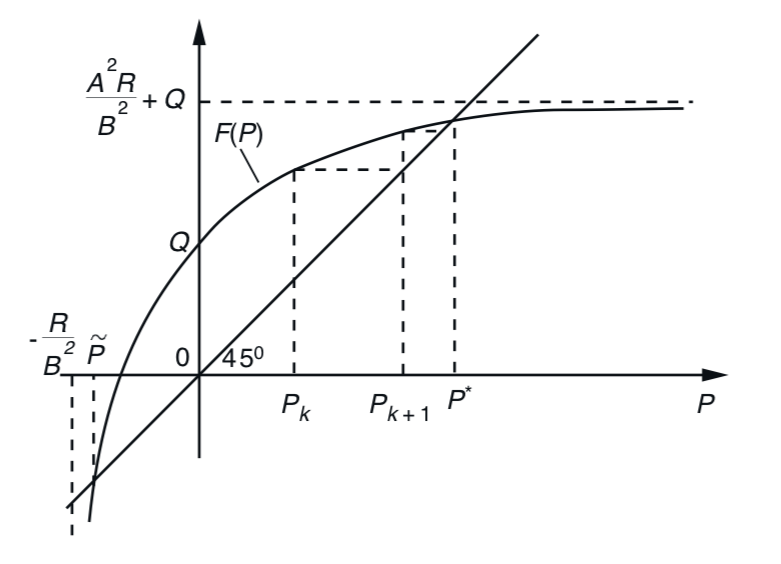
\includegraphics[width=0.6\textwidth]{Forth_lecture/p_6}
\caption{Graphical Proof For Scalar Systems}
\label{fig:3:1}
\end{figure}
\end{proof}
\paragraph{Random System Matrices}
Suppose that $\{A_0,B_0\},\dots,\{A_{N-1},B_{N-1}\}$ are not known but \emph{independent random matrices} that are also independent of the $\omega_k$. The DP algorithm is given by:
\begin{align*}
J_N(x_N)&=x_N\trans Q_Nx_N\\
J_k(x_k)&=\min_{u_k}\mathbb{E}_{\omega_k,A_k,B_k}
\left\{
x_k\trans Q_kx_k
+
u_k\trans R_ku_k
+
J_{k+1}(A_kx_k+B_ku_k+\omega_k)
\right\}
\end{align*}
Following the similar proof in Theorem~(\ref{The:3:1}), we imply
\[
\mu^*k(x_k) = L_kx_k,\ \text{where }
L_k
=-(R_k + \mathbb{E}\{B_k\trans K_{k+1}B_k\})^{-1}\mathbb{E}\{B_k\trans K_{k+1}A_k\}
\]
and the cost-to-go function $J_k(x_k) = x_k\trans K_kx_k+\text{constant}$, with
\begin{align*}
K_N&=Q_N\\
K_k&=\mathbb{E}\{A_k\trans K_{k+1}A_k\} - \mathbb{E}\{A_k\trans K_{k+1}B_k\}\\&(R_k + \mathbb{E}\{B_k\trans K_{k+1}B_k\})^{-1}\mathbb{E}\{B_k\trans K_{k+1}A_k\}+Q_k
\end{align*}
However, there are several drawbacks for random matrices systems:
\begin{enumerate}
\item
Certainty Equivalence may not hold (what is certainty equivalence?)
Formally speaking, the optimal controller may not be the same as for the corresponding deterministic problem, when the randomness is replaced by its expectation.
\item
Riccati equation may not converge to a steady-state.
\end{enumerate}
\begin{figure}
\centering
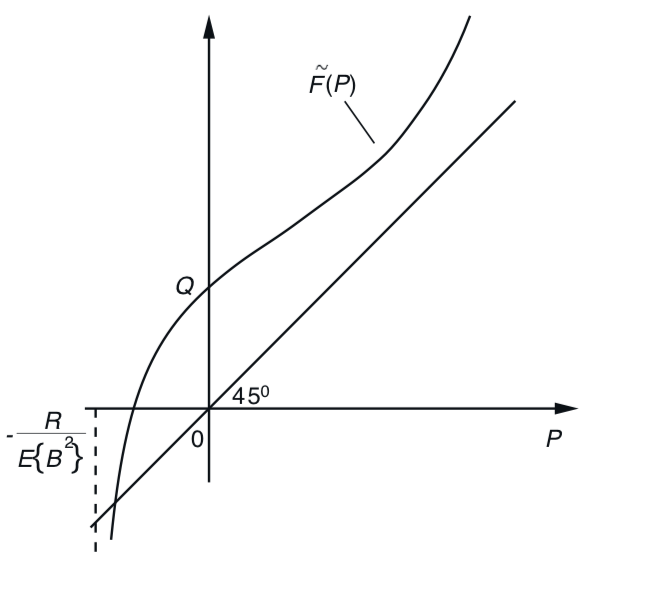
\includegraphics[width=0.6\textwidth]{Forth_lecture/p_7}
\caption{Graphical Illustration for a scalar stationary system}
\label{fig:3:2}
\end{figure}
Consider the scalar stationary system such that for the update for $K_{k+1}$, the random matrices $A_k,B_k$ are replaced by their expectation. Therefore, the update for $K_{k+1}$ can be written as
\[
\left\{
\begin{aligned}
K_{k+1}&=\tilde{F}(K_k)\\
\tilde{F}(K)&=\frac{\mathbb{E}\{A^2\}BK}{\mathbb{E}\{B^2\}K+R}+Q+\frac{TK^2}{\mathbb{E}\{B^2\}K+R}\\
T&=\mathbb{E}\{A^2\}\mathbb{E}\{B^2\} - (\mathbb{E}\{A\})^2(\mathbb{E}\{B\})^2
\end{aligned}
\right.
\]
When $T=0$, the problem reduces to the case where $A,B$ are not random; and we can obtain the well-studied asymptotic behavior; 
the convergece also happens as $T$ is small.
However, for large enough $T$, as shown in Fig~(\ref{fig:3:2}), the graph of $F$ do not intersect with the $45$-degree line on the positive interval, i.e., the Riccati equation diverges to infinity.


\section{Inventory Control}
\begin{itemize}
\item
State: inventory level $x_k$
\item
Control: number of orders $u_k$
\item
Disturbence: demand $\omega_k$
\item
System dynamics: $x_{k+1} = x_k + u_k -\omega_k$, $k=0,1,\dots,N-1$
\item
Stage cost:
\[
c\cdot u_k + H(x_k + u_k)
\]
where 
\[
H(x_k + u_k):=
\mathbb{E}_{\omega_k}
\left[
p\cdot(x_k+u_k-\omega_k)^- 
+
h\cdot(x_k+u_k-\omega_k)^+
\right]
\]
The goal is to minimize the total cost (question: do we need to add the expectation symbol?)
\[
\mathbb{E}\left\{\sum_{k=0}^{N-1}(cu_k + H(x_k+u_k))\right\}
\]
\end{itemize}

The dynamic programming algorithm applies as follows:
\begin{align*}
J_N(x_N)&=0\\
J_k(x_k)
&=
\min_{u_k\ge0}
\left[
c\cdot u_k
+
H(x_k+u_k)
+
\mathbb{E}_{\omega_k}
J_{k+1}(x_{k+1})
\right]
\end{align*}
\paragraph{Optimal Policy}
Regaring $y_k = x_k+u_k$ as the decision variable, it suffices to solve
\[
\begin{array}{ll}
\min_{y_k\ge x_k}&G_k(y_k) - cx_k,\\
\text{where }&G_k(y)
=cy+H(y)+\mathbb{E}_{\omega}\left[J_{k+1}(y-\omega)\right]
\end{array}
\]
\begin{proposition}\label{pro:3:1}
If $G_k$ is convex, and $\lim_{|x|\to\infty}G_k(x)\to\infty$, we have the optimal policy
\[
\mu_k^*(x_k) = \left\{
\begin{aligned}
S_k-x_k,\quad&\text{if }x_k<S_k\\
0,\quad&\text{if }x_k\ge S_k
\end{aligned}
\right.
\]
where $S_k$ is the minimizer of $G_k(y)$.
\end{proposition}
Now we show the assumption for proposition~(\ref{pro:3:1}) mostly holds. We need to add the assumption $c<p$, since otherwise it would never be optimal to order new iterms at the last period.
\begin{proposition}
Assume that $c<p$, then $J_k$ is convex for all $k$ and 
\[
\lim_{|x|\to\infty}J_k(x)\to\infty,\quad k=0,1,\dots,N-1
\]
\end{proposition}

\begin{proof}
\begin{figure}
\centering
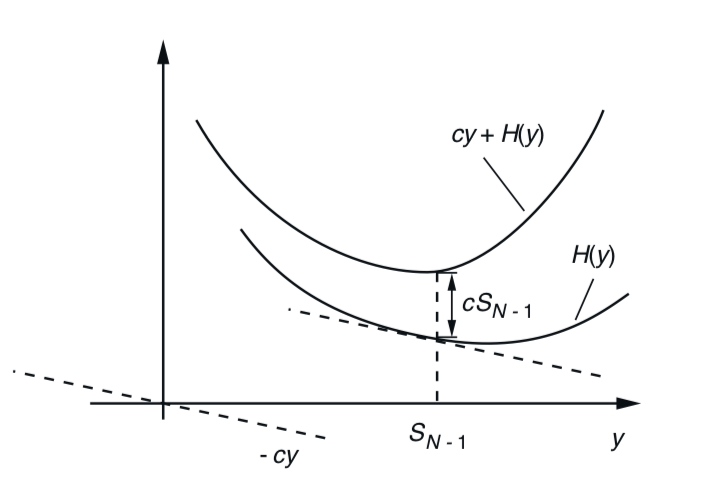
\includegraphics[width=0.6\textwidth]{Forth_lecture/p_8}
\caption{Graphical Illustration for the structure of cost-to-go function}
\label{fig:3:3}
\end{figure}
\begin{enumerate}
\item
It's easy to see that $J_N\equiv0$ is convex.
\item
Since $c<p$ and $H'(y)\to-p$ as $y\to-\infty$,
we imply that $G_{N-1}:=cy+H(y)$ has a derivative that becomes negative as $y\to-\infty$ and becomes positive when $y\to\infty$ (see Fig~(\ref{fig:3:3})). Therefore,
\[
\lim_{|y|\to\infty}G_{N-1}(y)=\infty.
\] 
As have shoen,
\[
\mu_{N-1}^*(x_{N-1})
=
\left\{
\begin{aligned}
S_{N-1} - x_{N-1},&\quad x_{N-1}<S_{N-1}\\
0,&\quad x_{N-1}\ge S_{N-1}
\end{aligned}
\right.
\]
Or equivalently, $\mu_{N-1}^*(x_{N-1})=(S_{N-1}-x_{N-1})^+$ (question: can we write in this form?). Substituting $\mu_{N-1}^*$ into $J_{N-1}$, we imply
\[
J_{N-1}(x_{N-1})=\left\{
\begin{aligned}
c\cdot(S_{N-1} - x_{N-1})+H(S_{N-1}),&\quad\text{if }x_{N-1}<S_{N-1}\\
H(x_{N-1}),&\quad\text{if }x_{N-1}\ge S_{N-1}
\end{aligned}
\right.
\]
which is clearly a convex function (question: why?)

Therefore, given the convexity of $J_N$, we are able to show the convexity of $J_{N-1}$. Furthermore,
\[
\lim_{|y|\to\infty}J_{N-1}(y)=\infty.
\]
\item
Similarly, given that $J_{k+1}$ is convex and $\lim_{|y|\to\infty}J_{k+1}(y)=\infty$, $\lim_{|y|\to\infty}G_k(y)=\infty$, for $k=N-2,\dots,0$, we imply
\[
J_k(x_k) = \left\{
\begin{aligned}
c\cdot(S_k - x_k)+H(S_k)+\mathbb{E}\{J_{k+1}(S_k - \omega_k)\},&\quad \text{if }x_k<S_k\\
H(x_k)+\mathbb{E}\{J_{k+1}(x_k-\omega_k)\},&\quad\text{if }x_k\ge S_k
\end{aligned}
\right.
\]
where $S_k$ is the unconstrained minimizer of $G_k$.
Moreover, we imply $J_k$ is convex, $\lim_{|y|\to\infty}J_k(y) = \infty$ and 
$\lim_{|y|\to\infty}G_{k-1}(y)=\infty$.
\end{enumerate}
\end{proof}

Therefore, we reduce the policy-based optimization into the pattern of finding the baseline $S_k$, i.e., a traditional parametric optimization problem.

\begin{proposition}
If the disturbance $\omega_k$ is i.i.d., then we imply the stationary optimal policy, i.e., the policy baseline $S_k^*$ becomes constant.
\end{proposition}

Now suppose further that 
\[
c(u_k)
=
\left\{
\begin{aligned}
K+c\cdot u_k,&\quad u_k>0\\
0,&\quad u_k=0
\end{aligned}
\right.
\]
Now the question is that do we obtain the pattern with baseline?
\begin{align*}
J_k(x_k)
&=
\min
[
\min_{u_k>0}
[K+cu_k+H(x_k+u_k)]+\mathbb{E}_{\omega_k}J_{k+1}(x_{k+1})\\
&,
0+H(x_k)+\mathbb{E}J_{k+1}(x_k)]\\
&=\min
\left[
\min_{y_k\ge x_j}(K+G_k(y_k)), G_k(x_k)
\right] - cx_k
\end{align*}
where $f(x_k):=\min_{y_k\ge x_j}(K+G_k(y_k))$ has its shape. Then we need to compare the two curves $f(x_k)$ and $G_k(x_k)$:
\[
u_k^*
=
\left\{
\begin{aligned}
S_k-x_k,&\quad\text{if }x_k\le S_k\\
0,&\quad\text{if }x_k>S_k
\end{aligned}
\right.
\]
\begin{itemize}
\item
If the inventory is very low (compare the baseline $s_k$), order $u_k^*=S_k-x_k$ to make the inventory into $S_k$
\item
If not that low, not order anything.
\end{itemize}
\begin{remark}
Unfortunately, $J_{k+1}(x_k)$ is convex does not necessarily imply $J_k(x_k)$ is convex. There is a concept $K$-convexity in literature. Under this $K$-convexity setting, we can show that the control $u_k^*$ still obtain the similar pattern but with two baselines, i.e., the decision can be made by first computing the baseline $(s,S)$, and then obtaining the $(s,S)$ strategy.
\end{remark}

The key for reducing computational complexity is to find patterns for decision variable $u_k^*$.

\section{Optimal Stopping Problem}
There are two possible controls for a stopping problem:
\begin{enumerate}
\item
Stop, i.e., incur a one-time stopping cost, and move to a \emph{cost-free}, \emph{absorbing} stop state.
\item
Continue, using $x_{k+1} = f_k(x_k,\omega_k)$ and incurring the \emph{cost-per-stage}
\end{enumerate}
Therefore, eacy policy should consist of a partition of a set of states $x_k$ into two regions:
\begin{enumerate}
\item
Stop region: where we stop?
\item
Continue region, where do we continue?
\end{enumerate}
The natural question is that can we obtain an optimal policy that is similar to the pattern of the \emph{baseline} studied in inventory control problem?




\paragraph{Asset Selling}
Suppose an industry wants to sell its iterms.
This industry receives a random price $\omega_k$ for $k=1,\dots,N-1$, which are assumed to be i.i.d. with known distribution. This industry may accept $\omega_k$ and invest the money at a fixed rate of interest $r$; or reject $\omega_k$ and wait for $\omega_{k+1}$. It must accept the last offer $\omega_{N-1}$

We may formulate this problem as follows:
\begin{itemize}
\item
State: $x_k=\omega_k$
\item
Decision variable: $u^1$ for sell and $u^2$ for wait.
\item
Stage reward:
\[
g(x_k,u_k,\omega_k)=\left\{
\begin{aligned}
x_k(1+r)^{N-1},\quad&\text{if }u_k=u^1\\
0,\quad &\text{if }u_k = u^2
\end{aligned}
\right.
\]
\item
Therefore, the DP algorithm is by solving the optimization problem below recursively:
\begin{align*}
J_N(x_N)&=\left\{
\begin{aligned}
x_N&\quad\text{if $x_N\ne T$}\\
0,&\quad\text{if $x_N=T$}
\end{aligned}
\right.\\
J_k(x_k)&=
\left\{
\begin{aligned}
\max\left[(1+r)^{N-k}x_k,\mathbb{E}\{J_{k+1}(\omega_k)\}\right]&\quad\text{if $x_k\ne T$}\\
0,&\quad\text{if $x_k=T$}
\end{aligned}
\right.
\end{align*}
\end{itemize}

Specifically, note that for $k$-th stage, if $x_k(1+r)^{N-k}\ge \mathbb{E}_{\omega_k}[J_{k+1}(\omega_k)]$, then the industry should decide to sell; otherwise decide to wait.

Define the variable (baseline)
\[
\alpha_k=\frac{\mathbb{E}J_{k+1}(\omega)}{(1+r)^{N-k}},
\]
then the optimal policy should be:
\[
\begin{array}{ll}
\text{accept the offer $x_k$}&\text{if $x_k>\alpha_k$}\\
\text{reject the offer $x_k$}&\text{if $x_k<\alpha_k$}
\end{array}
\]
In particular, the high baseline corresponds to the high standard for offering the price.

\paragraph{Future Analysis}
\begin{theorem}
Based on the assumption of i.i.d. $\omega_k$, the baseline $\alpha_k\ge\alpha_{k+1}$ for all $k$.
\end{theorem}
\begin{proof}
First introduce the functions
\[
V_k(x_k) = \frac{J_k(x_k)}{(1+r)^{N-k}},\qquad
x_k\ne T
\]
The DP algorithm reduces into 
\begin{align*}
V_N(x_N)&=x_N\\
V_k(x_k)&=\max\left[x_k,(1+r)^{-1}\mathbb{E}_{\omega}\{V_{k+1}(\omega)\}\right]
\end{align*}
Note that $\alpha_k = \mathbb{E}\{V_{k+1}(\omega)\}/(1+r)$. It's clear that
\[
V_{N-1}(x)\ge V_N(x),\quad\forall x\ge0
\]
Following the similar procedure, we derive $V_k(x)\ge V_{k+1}(x)$ for all $x$ and $k$. Since $\alpha_k = \mathbb{E}\{V_{k+1}(\omega)\}/(1+r)$, we obtain $\alpha_k\ge\alpha_{k+1}$, as desired.

\end{proof}
\begin{remark}
We can also show that $\alpha_k\to\bar{\alpha}$ as $k\to\infty$, where $\bar{\alpha}$ is a constant satisfying
\[
(1+r)\bar{\alpha} = P(\bar{\alpha})\bar{\alpha}+\int_{\bar{\alpha}}^\infty\omega \diff P(\omega)
\]
Therefore, for an infinite horizon, the optimal policy is stationary.
\end{remark}



Now we show that $\{\alpha_k\}$ is monotonically decreasing.

Define 
\[
V_k(x_k) = \frac{J_k(x_k)}{(1+r)^{N-k}}
\implies
V_k(x_k) = \max\left(x_k,\frac{\mathbb{E}V_{k+1}(\omega)}{1+r}\right)
\]
and $V_N(x_N) = x_N$.

Note that we show $V_{k+1}(x)\le V_k(x)$ first:
\begin{align*}
V_N(x)&=x\\
V_{N-1}(x)&=\max(x,\mathbb{E}V_N(\omega))
\end{align*}
It's clear that $V_N(x)\le V_{N-1}(x)$.
\begin{align*}
V_K(x)&=\max(x,\frac{\mathbb{E}V_{k+1}(\omega)}{1+r})\\
V_{k-1}(x)&=\max(x,\frac{\mathbb{E}V_{k}(\omega)}{1+r})
\end{align*}
It's clear that $V_k(x)\le V_{k-1}(x)$ for any $k$. Therefore,  $\{\alpha_k\}$ is monotonically decreasing.

Note that the key for this proof is the i.i.d. of $\omega_k$.

\begin{itemize}
\item
Pattern
\item
Trends
\item
Convergence: If there are inifinte horizons, what is the bottleneck for the policy.
\end{itemize}

In this case,
\begin{equation}\label{Eq:3:1}
\begin{aligned}
\alpha_k &= \frac{\mathbb{E}V_{k+1}(\omega)}{1+r}
=
\frac{1}{1+r}
\left[\int_0^{\alpha_{k+1}}\alpha_{k+1}d P(\omega)
+
\int_{\alpha_{k+1}}^\infty \omega d P(\omega)
\right]\\
&=\frac{P(\alpha_{k+1})}{1+r}\alpha_{k=1}
+
\frac{1}{1+r}\int_{\alpha_{k+1}}^\infty\omega d P(\omega)
\end{aligned}
\end{equation}
where the $P(\alpha_{k+1})$ is the cdf, and $\alpha_k$ is bounded.


Start from $\alpha_N=0$, derive $\alpha_{N-1},\dots,\alpha_0$ sequentially.

When $N\to\infty$, note that computing the equation above is based on the derivation of $\alpha_{N+1}$. We can imply the convergence of $\alpha$, and we can compute $\alpha_{N+1}$ based on (\ref{Eq:3:1}).








